\begin{figure*}[!ht]
    \centering
    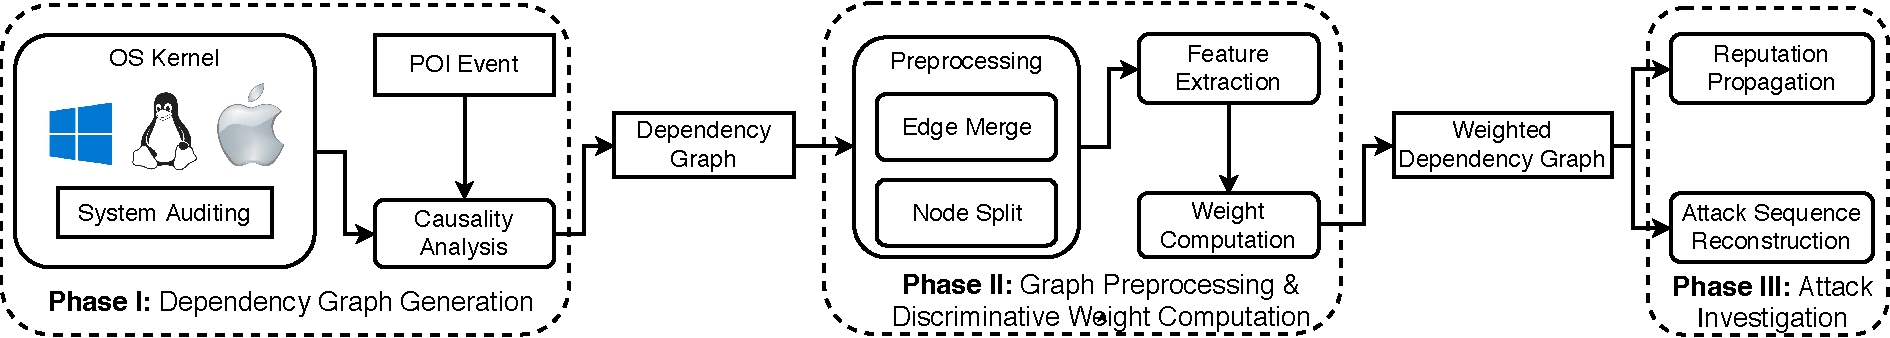
\includegraphics[width=0.95\textwidth,clip]{figs/architecture.pdf}
  %  \vspace{3mm}
    \caption{The architecture of \tool}
  %  \vspace{2mm}
    \label{fig:overview}
%    \vspace*{-1ex}
\end{figure*}


\section{Overview and Threat Model}
\label{sec:overview}

% https://drive.google.com/file/d/1HKHxWAoQWrw-ZGfvF3AJuEUhGcIF-BCy/view?usp=sharing
\cref{fig:overview} illustrates the architecture of \tool. 
\tool consists of three phases: (1) dependency graph generation, (2) graph preprocessing \& discriminative weight computation, and (3) attack investigation.
In Phase I, 
\tool leverages mature system auditing tools (\eg auditd~\cite{auditd}, ETW~\cite{etw}, DTrace~\cite{dtrace}, and Sysdig~\cite{sysdig}) to collect system-level audit logs about system calls.
Given a POI event, \tool parses the collected logs and performs causality analysis~\cite{backtracking,backtracking2} to generate the dependency graph for the event (\cref{subsec:graph-generation}).
%
In Phase II, \tool preprocesses the graph by merging the same type of edges between two nodes that occur within a time window threshold to reduce the graph size and splitting the nodes to remove parallel edges. 
This process transforms the large dependency graph into a simple directed graph (\cref{subsec:graph-preprocessing}), which is easier for weight computation and reputation propagation.
To compute discriminative weights for edges so that critical edges can be easily revealed from non-critical edges,
%To produce a weighted dependency graph such that critical edges
%(\ie edges that reveal the attack provenance) 
%can be easily revealed from non-critical edges using their edge weights, 
for each edge, \tool extracts three novel features that model the 
%importance of the event edge with respect to the POI event
%correlation between the event edge and the POI event 
impact of the event edge on the POI event
from three aspects: time aspect, data amount aspect, and structure aspect (\cref{subsec:feature-extraction}). 
\tool then employs a novel 
\emph{discriminative feature projection scheme}
%\emph{local feature projection mechanism}
to combine the three features into a single discriminative weight (\cref{subsec:weight-computation}).
%
%
In Phase III, \tool propagates reputation from entry nodes to the POI along the weighted edges to infer the POI reputation.
The 
%inferred 
POI reputation will be used to identify the root cause nodes and determine the POI trustworthiness/suspiciousness. 
Furthermore, \tool provides a suggested range of threshold values based on the edge weights, which will be used to reconstruct the attack sequence.





\myparatight{Threat Model}
Our threat model follows the threat model of previous work on system monitoring~\cite{backtracking,backtracking2,loggc,trustkernel,gao2018aiql,gao2018saql,liu2018priotracker,hassan2019nodoze}. 
We assume that the system monitoring data collected from kernel space~\cite{auditd,etw,dtrace,sysdig} is not tampered, and that the kernel is trusted.
Any kernel-level attack that deliberately compromises security auditing systems is beyond the scope of this work.



\eat{
The attacker executes APT attacks involving multiple steps such as target discovery and data exfiltration. We assume an outside attacker that attacks the system remotely (from outside of the system). Thus, the attacker either utilizes the vulnerabilities in the system or convinces the user to download a file. The main goal of the attacker is to inject her malicious files into the victim’s system without being detected. In this work, we assume the attacker does not know how the proposed reputation system operates, and hence we do not consider the potential attacks against the reputation system. 

% We do consider that insiders or external attackers have full knowledge of the deployed \tool queries and the anomaly models. 
}
